\documentclass[12pt]{article}
\setlength{\oddsidemargin}{0in}
\setlength{\evensidemargin}{0in}
\setlength{\textwidth}{6.5in}
\setlength{\parindent}{0in}
\setlength{\parskip}{\baselineskip}
\usepackage{amsmath,amsfonts,amssymb}
\usepackage{graphicx}
\usepackage[]{algorithmicx}
\usepackage{enumitem}
\usepackage{fancyvrb}
\usepackage{ wasysym }
\usepackage{tkz-berge}
\usetikzlibrary{positioning, automata}

\usepackage{pgf}

\usepackage{tikz}

\usetikzlibrary{arrows,automata}

\usepackage[latin1]{inputenc}

\usepackage{fancyhdr}
\pagestyle{fancy}
\setlength{\headsep}{36pt}

\usepackage{hyperref}


\hypersetup{
    colorlinks=true,
    linkcolor=blue,
    filecolor=magenta,      
    urlcolor=blue,
}

\newcommand{\makenonemptybox}[2]{%
%\par\nobreak\vspace{\ht\strutbox}\noindent
\item[]
\fbox{% added -2\fboxrule to specified width to avoid overfull hboxes
% and removed the -2\fboxsep from height specification (image not updated)
% because in MWE 2cm is should be height of contents excluding sep and frame
\parbox[c][#1][t]{\dimexpr\linewidth-2\fboxsep-2\fboxrule}{
  \hrule width \hsize height 0pt
  #2
 }%
}%
\par\vspace{\ht\strutbox}
}
\makeatother

\begin{document}
\lhead{{\bf CSCI 3104, Algorithms \\ Homework 6 (100 points)} }
\rhead{Name: \fbox{% Place your name here and delete the next time
\phantom{This is a really long name}} 
\\ ID: \fbox{ % Place your ID here and delete the next time
\phantom{This is a student ID}} 
\\ {\bf Escobedo \& Jahagirdar\\ Summer 2020, CU-Boulder}}
\renewcommand{\headrulewidth}{0.5pt}

\phantom{Test}

\begin{small}
\textit{Advice 1}:\ For every problem in this class, you must justify your answer:\ show how you arrived at it and why it is correct. If there are assumptions you need to make along the way, state those clearly.
%\vspace{-3mm} 

\textit{Advice 2}:\ Verbal reasoning is typically insufficient for full credit. Instead, write a logical argument, in the style of a mathematical proof.\\
%\vspace{-3mm} 

\textbf{Instructions for submitting your solution}:
\vspace{-5mm} 

\begin{itemize}
	\item The solutions \textbf{should be typed}, we cannot accept hand-written solutions. Here's a short intro to \href{http://ece.uprm.edu/~caceros/latex/introduction.pdf}{\textbf{Latex}.}
	 \item In this homework we denote the asymptomatic \textit{Big-O} notation by $\mathcal{O}$ and \textit{Small-O} notation is represented as $o$. 
	\item We recommend using online Latex editor \href{https://www.overleaf.com/}{\textbf{Overleaf}}. Download the \textbf{.tex} file from Canvas and upload it on overleaf to edit.
	%todo add link of gradescope
	\item You should submit your work through \href{https://www.gradescope.com}{\textbf{Gradescope}}  only.
	\item If you don't have an account on it, sign up for one using your CU email. You should have gotten an email to sign up. If your name based CU email doesn't work, try the identikey@colorado.edu version. 
	\item Gradescope will only accept \textbf{.pdf} files (except for code files that should be submitted separately on Canvas if a problem set has them) and \textbf{try to fit your work in the box provided}. 
	\item You cannot submit a pdf which has less pages than what we provided you as Gradescope won't allow it.
   
\end{itemize}
\vspace{-4mm} 
\end{small}

\hrulefill
\pagebreak

\subsection*{Piazza threads for hints and further discussion}
\begin{center}
    \begin{tabular}{|c|}
    \hline
    Piazza Threads \\ [0.5ex] 
    \hline \hline 
    \href{https://piazza.com/class/ka2roz7rb9m3j4?cid=87}{Question 1}\\
    \href{https://piazza.com/class/ka2roz7rb9m3j4?cid=88}{Question 2}\\
    \href{https://piazza.com/class/ka2roz7rb9m3j4?cid=89}{Question 3}\\
    \href{https://piazza.com/class/ka2roz7rb9m3j4?cid=90}{Question 4}\\
    \href{https://piazza.com/class/ka2roz7rb9m3j4?cid=91}{Question 5}\\
    \href{https://piazza.com/class/ka2roz7rb9m3j4?cid=92}{Question 6}\\
    \href{https://piazza.com/class/ka2roz7rb9m3j4?cid=93}{Question 7}\\
    \href{https://piazza.com/class/ka2roz7rb9m3j4?cid=94}{Question 8}\\
    \hline
    \end{tabular}
\end{center}

\textbf{Recommended reading}: \\
Graph Algorithms Intro: Ch. 22 $\to$ 22.1, 22.2, 22.3 \\
Graph Algorithms SSSPs: Ch. 24 $\to$ 24.3
\\

\pagebreak

\begin{enumerate}
    
     \item (5 pts) How many unique MSTs does the following graph have. Show the necessary work to justify your answer. 
    \begin{figure}[h!]
    \begin{center}
    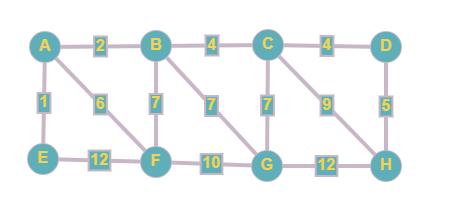
\includegraphics[scale=1]{/home/satyam/1594704015-Archive/p1.PNG} 
    \end{center}
    \end{figure}
    \makenonemptybox{4in}{There are 2 unique MST. Since edge to G either from vertices B or C is having weight of 7. Either one of the edges can be choosen. While all the remaining path are distinct, we will have to pick minimum of the edges weight. If the edge of BF is choosen, it leads to cycle formation, which is not permissible. Hence this edges is not choosen and also it will not result in MST. }

    \item (20 pts) Based on the following graph :
    \begin{figure}[h!]
    \begin{center}
    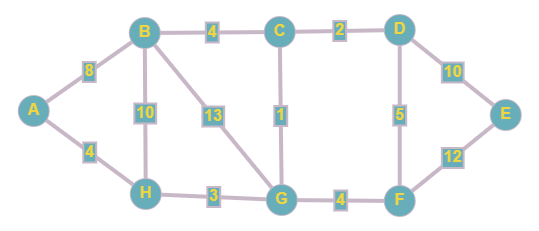
\includegraphics[scale=1]{/home/satyam/1594704015-Archive/p2.png} 
    \end{center}
    \end{figure}

    \begin{enumerate}[label=(\alph*)]
        \item (10 pts) In what order would Prim's algorithm add edges to the MST if we start at     vertex $A$? 
        \makenonemptybox{3in}{ There are 2 possible of MST using Prim's Algorithm, Since edge C-B and G-F have equal weights of 4, so either of the edge can be selected:\begin{enumerate}
        		\item .Order from A-H-G-C-D-B-F-E (If vertex B is selected first)
        		\item Order from A-H-G-C-D-F-B-E (If vertex F is selected first)
        	\end{enumerate}
        	
         }
        \clearpage
        \item (10 pts) In what order Kruskal's would add the edges to the MST? 
        \makenonemptybox{6in}{First sort all the edge weight in ascending order.
        Edge weights are \{1,2,3,4,4,4,5,8,10,10,12,13\}. 
        \begin{itemize}
        	\item Selecting vertices with minimum edge weights, Assume C is selected as the starting vertex and edge C-G is visited. Vertex C,G is added into set. 
        	\item Selecting D as the next vertex and it is added into the set.Order : \{C,G,D\}
        	\item Selecting H as the next vertex and it is added into the set.Order : \{C,G,D,H\}
        	\item There are 3 edges with edge weights as 4, so there can 3!=6 possible order in Kruskal.  One of the possible order is selecting first A as the next vertex. Vertices  B or F are added in any order.  Order : \{C,G,D,H,A,B,F\} or  \{C,G,D,H,A,F,B\}
        	\item  Another possibility is adding vertex B (assume to be first vertex selected with equal wieghts) into the set and A,F in any order. Order:  \{C,G,D,H,B,A,F\} or \{C,G,D,H,B,F,A\}
        	\item  Another possibility is adding vertex F (assume to be first vertex selected with equal wieghts) into the set and A,B in any order. Order : \{C,G,D,H,F,A,B\} or \{C,G,D,H,F,B,A\}
        	\item Adding E, with edge from D-E into the set.
        	
        \end{itemize} 
         Order of Kruskal's Algorithm (All 6 possibilities)
         \begin{enumerate}
         	\item  \{C,G,D,H,A,B,F,E\}
         	\item   \{C,G,D,H,A,F,B,E\}
         \item	\{C,G,D,H,B,A,F,E\}
         \item  \{C,G,D,H,B,F,A,E\}
         \item  \{C,G,D,H,F,A,B,E\}
         \item \{C,G,D,H,F,B,A,E\}
         \end{enumerate}
         
    
}
    \end{enumerate}
    \clearpage
    
    \item (10 pts) Suppose that you have calculated the MST of an undirected graph $G=(V,E)$ with positive edge weights.  If you increase each edge weight by 5, will the MST change? Prove that it cannot change or give a counterexample if it changes. (Note: Your proof, if there is one, can be a simple logical argument.)
  
    \makenonemptybox{6in}{Consider a graph with $G=(V,E)$ and edge weights(w(i,j)) $\geq$0 and i,j $\in$ E. The new weight becomes w'(i,j)) +5 i,j $\in$ E. MST will not change. \\ \\
   Assume the graph $G$ has $n$ vertices, then any spanning tree of $G$ will have $n−1$ edges.  $\therefore$ incrementing each edge weight by 5 increases the cost of every spanning tree by a constant$times$(n−1).  So any spanning tree with minimal cost in the original graph also has minimal cost in the new graph with increased weights.}
	\clearpage

    \item (15 pts) Suppose you are given the minimum spanning tree $T$ of a given graph G (with $n$ vertices and $m$ edges) and a new edge $e=(u,v)$ of weight $w$ that will be added to $G$. Give an efficient algorithm to find the MST of the graph $G\cup e$. Your algorithm should run in $O(n)$ time.\\
	\makenonemptybox{6in}{ Addition of an edges to the graph creates one cycle. Examine the path of the spanning tree T from u to v (either using DFS or BFS) . If any vertex on this path has weight larger than that of the new edge, then T is no longer an MST. The spanning tree is modified in such a way so that   max weight edge on this path is removed  and replace it with the new edge. The runtime of this algorithm is $O(n)$.
	
}
	\clearpage

    
    
    \item (20 pts) 
    In a directed graph $G=(V, E)$ with positive edge weights, we define the maximum weight of a path from $s$ to $t$ to be the maximum of the edge weights along the path. For example, if the path from $s$ to $t$ has edges with weights $e_1 = 10, e_2 = 15, e_3 = 5$ then the maximum of the path is $max(e_1, e_2, e_3) = 15$. Give an algorithm to compute the smallest maximum weight paths from a source vertex $s$ to all other vertices. (Hint:  Your algorithm should be a modification of Dijkstra’s algorithm)
    \makenonemptybox{6in}{To compute min(max($e_{1},e_{2}\cdots e_{n}$))\\
The idea is to use Dijkstra’s algorithm. In order to find the longest/maximum path from a given vertex to a given destination vertex we reverse all the edges of the directed graph and let this graph be $G'=(V,E')$. The source and destination remains same as the graph $G$. Since all the edges are now reversed computing the longest/maximum distance from the destination vertex. After finding the maximum distance, finding minimum among all the edges, if more than 1 path exists from destination to source exists.\\
Time complexity: $O(V+E)$ (can be implemented using priority queue).
\\Space complexity: $O(V)$
}
	\clearpage
    
    \item (2 pts) What are the two conditions that must be met for the flow on a graph to be valid?
    \makenonemptybox{2in}{ A flow graph is directed multigraph Graph $G=(V,E)$ and the capacity of the flow network $> 0$ and denoted by c.
    	Following two properties that a flow must satisfy:
    	\begin{enumerate}
    		\item 	Capacity constraint: $\forall$ edges in a graph, flow in the network must be $\leq$ to c.
\item 	Flow conservation: $\forall$ vertex $\in$ $V-\{source,sink\}$, flow of the edges must be equal ie incoming flow and outcoming must be equal for the edges.\\

When the edges $\notin$ E, there is no flow in the network(ie the vertex is source).
    	\end{enumerate}
    
    }
	


\item (3 pts) What do the edge weights in the residual graph $G_f$ represent? Include the definition of both forward and backward edges.
\makenonemptybox{2in}{edge weights in the residual graph $G_f$ represents amount of flow, which can be added  to the network and it must be equal to edge’s capacity minus the flow on that edge. \\Assume s $\in$$ V_{s}$ and t$\in$$ V_{t}$, where s is the source and t is the sink. An edge that goes from vertex u  to  v  is  a  forward  edge  if  u $\in$$V_{s}$ and v $\in$ $V_{t}$. Vice Versa is the backward edge.
	Flow  at  each  forward  edge  is  to  its  capacity and the flow at each backwards edge is 0}
    
    \clearpage
    \item (25 pts) Based on the following network and the given edge capacities answer the following. 
\begin{figure}[h!]
\begin{center}
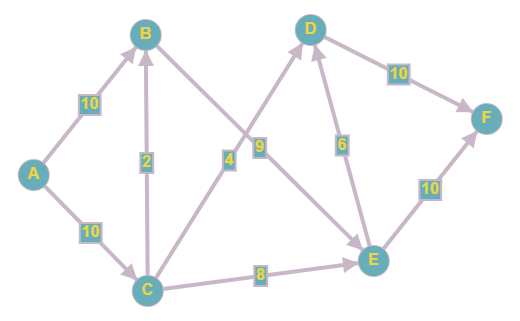
\includegraphics[scale=0.7]{/home/satyam/1594704015-Archive/p8.png}
\end{center}
\end{figure}

\begin{enumerate}
\item (15 pts) Suppose we start the Ford-Fulkerson algorithm  with  $\textbf{A}$ being the source vertex and $\textbf{F}$ being the sink and \textbf{select the path $A ->C ->B -> E -> D ->F$ in the first iteration (Do not chose the first A-F path on your own).} Complete all the iterations of Ford-Fulkerson to find the Max-Flow (including the first round that is incomplete).
Clearly show each round with \\
\begin{enumerate}
\item The path that you are selecting in that round.
\item The bottleneck edge on this path.
\item The additional flow that you push from the source by augmenting (pushing maximum allowed flow along) this selected augmenting path.
\item The residual graph with the residual capacities (on both the forward and backward) edges.
\end{enumerate}
Also, report the Max-Flow after the algorithm terminates.

\makenonemptybox{6in}{\begin{center}

		\begin{tabular}{ |p{0.5cm}| p{5.5cm}| c| c| }

			
		\hline
			Itr & Path (i) & Bottleneck Edge(ii) & Capacity (iii) \\ 
\hline
		1 & $A->C->B-> E-> D->F$ & C-B & 2 \\ \hline
		2 & $A ->B-> E ->F$ & B-E & 7 \\ \hline
		3 & $A ->C -> D ->F$ & C-D & 4 \\ \hline
		4 & $A ->C -> E ->F$ & E-F & 3 \\ \hline
		5 & $A ->C -> E -> D ->F$ & D-F & 1 \\  \hline
   

		\end{tabular}

	\end{center}
(iv) Residual Capacities on path (ACBEDF) are $A--(8)->C--(0)-->B--(7)--> E-- (4)--> D --(8)-->F$  \\
Residual Capacities on path (ABEF) are $A--(3)-->B--(0)--> E--(3)-->F$  \\
Residual Capacities on path (ACDF) are $A--(4)->C-- (0)--> D --(4)-->F$  \\
Residual Capacities on path (ACEF) are $A--(1)->C--(5)--> E--(0)-->F$  \\
Residual Capacities on path (ACEDF) are $A--(0)->C--(4)--> E-- (3)--> D --(3)-->F$  \\  

Maximum flow capacity = 17
}
\clearpage

\item (5 pts) Draw the graph and show the final flow f(e) for the edges of the original graph when the Ford-Fulkerson algorithm terminates.
%\makenonemptybox{3in}
\begin{figure}[h!]
	\begin{center}
		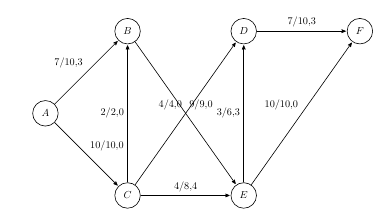
\includegraphics[scale=0.7]{/home/satyam/1594704015-Archive/HW61.png}
	\end{center}
\end{figure}
\item (5 pts) Find the minimum capacity cut with respect to the capacities on the original graph. Is this minimum capacity equal to the Max-Flow that you earlier identified? Justify your answer in a sentence. Also, list the  edges that are part of the min-cut and are saturated (can't carry any more flow).
\makenonemptybox{3in}{Path: A-C-E-D:10+4+3=17(Out of 8 units,only 4 units can flow from C-E, 3 units can flow from E-D.). Maximum flow is equal to minimum capacity cut. A-C edges are saturated as all the flow is consumed by the C.}
\end{enumerate}

\item{\itshape \textbf{Extra Credit Question 1 (5 pts)}
    For this extra credit question, please refer the leetcode link provided below or click \href{https://leetcode.com/problems/cheapest-flights-within-k-stops/}{here}. Multiple solutions exist to this question ranging from brute force to the most optimal one. Points will be provided based on Time and Space Complexities relative to that of the most optimal solution.

    Please provide your solution with proper comments which carries points as well.}
    
   \url{https://leetcode.com/problems/cheapest-flights-within-k-stops/}

    % Paste your code in the verbatim tag below
\begin{verbatim}
class Solution {

public:


struct cmp {

bool operator()(const vector<int> &a, const vector<int> &b) {

return a[1] > b[1];                          //Return the lesser distanc of the 2.

}                                            //Remember preiority queue is maxheap by default

};


int findCheapestPrice(int n, vector<vector<int>>& flights, int src, int dst, int K) {

priority_queue<vector<int>, vector<vector<int>>, cmp> pq;      //We use a minheap to select the minimum distance

vector<pair<int,int>> adj[n];

for (int i=0;i<flights.size();i++) {

adj[flights[i][0]].push_back(make_pair(flights[i][1], flights[i][2]));   //Our adjacency list consists of sorce,destination,distance

}


for(int i=0;i<adj[src].size();i++) {

vector<int> vec({adj[src][i].first, adj[src][i].second, 0});      //Our priority queue consists of destination,distance,no of stops

pq.push(vec);

}

if(pq.empty())                                        //If pq is empty there are no routes from souce thus return -1

return -1;


while (!pq.empty())

{

vector<int> p = pq.top();

pq.pop();


if (p[2] > K)    //If the number of stops is greater than k we just pop the element and analyze the next element

continue;

if(p[0] == dst)  //If the destination is reached we just return the distance calculated thus far

return p[1];


for(int i=0;i<adj[p[0]].size();i++) {

vector<int> vec({adj[p[0]][i].first, adj[p[0]][i].second + p[1], p[2] + 1});  //We add the currnt distance to the previous calculated one and increment the number of stops

pq.push(vec);

}


}

return -1;

}


};
\end{verbatim}	

\item{\itshape \textbf{Extra Credit Question 2 (5 pts)}
    For this extra credit question, please refer the leetcode link provided below or click \href{https://leetcode.com/problems/pacific-atlantic-water-flow/}{here}. Multiple solutions exist to this question ranging from brute force to the most optimal one. Points will be provided based on Time and Space Complexities relative to that of the most optimal solution.

    Please provide your solution with proper comments which carries points as well.}
    
   \url{https://leetcode.com/problems/pacific-atlantic-water-flow/}

    % Paste your code in the verbatim tag below
\begin{verbatim}
Replace this text with your source code inside of the .tex document
\end{verbatim}	

\end{enumerate}
\end{document}


